\subsection{Movimiento vertical}
\label{sec:mov_vertical_prototipo}

El sistema de movimiento vertical se basa en un mecanismo de varilla roscada trapezoidal acoplada a un motor paso a paso. A continuación se detallan las especificaciones de diseño:

\begin{itemize}[label=$\bullet$]
    \item Diámetro de varilla roscada: $d = 8$ mm
    \item Paso de rosca: $p = 8$ mm
    \item Longitud total de las varillas: $L = 1000$ mm
    \item Tipo de rosca: Trapezoidal
    \item Masa total a trasladar: $m_{total} = 1$ kg
\end{itemize}

Teniendo en cuenta una carga de 1kg se tiene que la fuerza es F=9.8 N. \\

El torque necesario en el husillo es el máxmio entre el torque de subida (ec. \ref{eq:torque_subida}) y el torque de bajada (ec. \ref{eq:torque_bajada}):

\begin{equation}
T_{subida}= 0.056\text{Nm}
\end{equation}

\begin{equation}
T_{bajada}= 0.035 \text{Nm}
\end{equation}
Considerando un factor de seguridad por fricción en roscas trapezoidales (\(f_1=2.5\)) y un factor de seguridad por torque dinámico (\(f_2=1.3\))
Se tiene que el torque total es: 
\[T_{motor}=f_1 \cdot f_2 \cdot MAX(T_{subida}, T_{bajada})= 0.182Nm\]

Se define la velocidad máxima como $v = 75$ mm/s y la aceleración máxima $a = 45$ mm/s$^2$, luego las revoluciones del motor son:
\[n= \frac{ 75 \frac{mm}{s} \cdot 60}{8 \frac{mm}{rev}}=562.5 rpm\]

\subsubsection{Selección del motor}

Se selecciona un motor paso a paso NEMA 23 con una alimentación de 24v, 4.5A y un torque de retención de 1.1 \(N \cdot m\).

\begin{figure}[H]
    \centering
    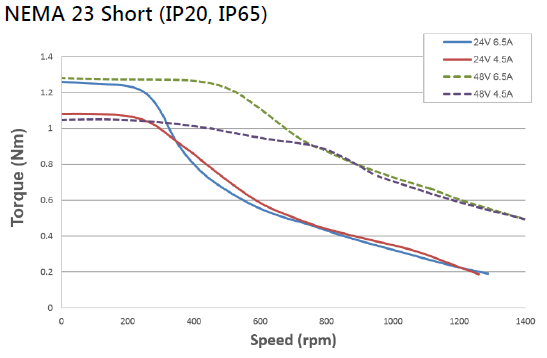
\includegraphics[width=0.65\textwidth]{img/nema23_proto.png}
    \caption{\textit{Curva dinámica torque-velocidad del motor paso a paso NEMA 23 para el prototipo.}}
    \label{fig:Curva_din_nema17medium}
\end{figure}

Como se puede observar, para aproximadamente 600rpm se cumple con el torque requerido.\\

\subsubsection{Justificación del diámetro de varilla}

\underline{Análisis de pandeo}\\
Para una varilla con longitud de 1000 mm sometida a carga axial, se debe verificar que no sufra pandeo. La carga crítica de Euler es:

\begin{equation}
P_{cr} = \frac{\pi^2 E I}{(K L)^2}
\end{equation}

donde:
\begin{itemize}[label=$\bullet$]
    \item $E = 200$ GPa (módulo de elasticidad del acero)
    \item $I = \frac{\pi d^4}{64} = \frac{\pi (0.008)^4}{64} = 2.01 \times 10^{-10}$ m$^4$
    \item $K = 1$ (factor de longitud efectiva, ambos extremos con rodamientos)
    \item $L = 1.0$ m
\end{itemize}

\begin{equation}
P_{cr} = \frac{\pi^2 \times 200 \times 10^9 \times 2.01 \times 10^{-10}}{(1.0)^2} = 397 \text{ N}
\end{equation}

El factor de seguridad contra pandeo:
\begin{equation}
FS_{pandeo} = \frac{P_{cr}}{F_{total}} = \frac{397}{21.63} = 18.36
\end{equation}

La tensión axial en la varilla:
\begin{equation}
\sigma = \frac{F_{total}}{A} = \frac{21.63}{\pi (0.004)^2} = \frac{21.63}{5.03 \times 10^{-5}} = 430 \text{ kPa}
\end{equation}

Para acero con límite elástico típico de $\sigma_y = 250$ MPa:
\begin{equation}
FS_{tensión} = \frac{\sigma_y}{\sigma} = \frac{250 \times 10^3}{0.43} = 581
\end{equation}

La deflexión máxima bajo carga:
\begin{equation}
\delta = \frac{F_{total} L}{A E} = \frac{21.63 \times 1.0}{5.03 \times 10^{-5} \times 200 \times 10^9} = 2.15 \times 10^{-6} \text{ m} = 0.002 \text{ mm}
\end{equation}

Esta deflexión es despreciable (< 0.01\% de la longitud total).

\underline{Velocidad crítica de rotación}
Para evitar resonancia, se verifica la velocidad crítica:
\begin{equation}
n_{cr} = \frac{30}{\pi L^2} \sqrt{\frac{E I}{\rho A}} \approx 3600 \text{ RPM}
\end{equation}

La velocidad de operación ($\approx$ 600 RPM) está muy por debajo de la velocidad crítica, garantizando operación estable.

\begin{itemize}[label=$\bullet$]
    \item La varilla roscada de 8 mm de diámetro con paso de 8 mm está correctamente dimensionada:
    \begin{itemize}[label=$\bullet$]
        \item Factor de seguridad contra pandeo: 18.36
        \item Factor de seguridad contra tensión: 581
        \item Deflexión bajo carga: < 0.003 mm (despreciable)
        \item Velocidad de operación muy inferior a la velocidad crítica
    \end{itemize}
    %\item El driver TB6600 configurado a 24V proporciona la corriente y voltaje necesarios para mantener el torque requerido a la velocidad de operación.
\end{itemize}